\documentclass[../../../main.tex]{subfiles}

\begin{document}

When I arrived at Whittier College in Fall 2017, my department had arranged my schedule such that I did not serve on a committee for the first year.  By Fall 2018, I had developed the idea that I could serve Whittier College by utilizing my skills in data analysis.  I was also interested in the connection between the high school preparation of our students and their ability to pass mathematics courses once we accepted them.  I had noticed a pattern in some of my introductory courses that some students had never been exposed to algebra, and that made it very difficult for them to pass courses required for their major.  After signing up for the Enrollment and Student Affairs Committee (ESAC), in Fall 2018, I learned that this is a sensitive topic with which many administrators and intructors had been struggling.

\subsection{Enrollment and Student Affairs Committee, Years 1 and 2}

I joined ESAC in Fall 2018, and our charge included the creation of recommendations for altering admissions criteria, discussing the criteria for athletics participation for students on probation, and organizational issues surrounding the orientation program and the creation of INTD101.  Our committee chair was Prof. Ayesha Shaikh.  Early in the year, Prof. Shaikh formed a sub-committee on admissions data analysis.  I volunteered to partipate with Prof. Charles Hill, and the vice president of enrollment (at the time) Kieron Miller was also included.  Working with Fritz Smith and others, we gathered educational data on several thousand students going back six years to examine what leads to the admission of students that do not join us again in the Fall of their sophomore year.
\\
\vspace{0.25cm}
The admissions data sub-committee met several times in person in Fall 2018.  Our discussions were broad at first, focusing on the the balance between admitting enough students with the need to admit students we know we can support and retain.  I did not always understand the contex of these conversations; adminstrators and professors more experienced than me seemed to be speaking more frankly in sub-committee, but in coded language in the main meeting.  ESAC had members from all aspects of the college participating, including admissions staff, the athletics director, members of CAAS, and professors from different divisions.  Eventually we received archived data in the form of spreadsheets for $N \approx 3,000$ students in their first two semesters at Whittier College.  I found a number of interesting effects regarding student GPA, standardized test scores, the financial aid gap, and student retention through the Fall semester of their sophomore year.  I presented my findings twice in front of the whole ESAC committee\footnote{These presentations are included in the supporting material.}.
\\
\vspace{0.25cm}
In my first presentation, I began with the basic finding that student GPAs during their first semester at Whittier College are not normally-distributed.  Given a random sample from a population of students, one expects a normal distribution (bell curve).  Figure \ref{fig:grade} is what we observed, after limiting the analysis to just the students for which we had all pieces of data ($N = 1,346$).  The fitted curves to the data points follow normal distributions.  There is a clear set of outliers on the left side each graph.  The left plot corresponds to the \textit{normalized} GPA distribution of Whittier College students in their first Fall semester.  Normalized GPA is just the GPA minus the average GPA, divided by the standard deviation in GPA.  Thus, a value of zero in Fig. \ref{fig:grade} simply means those are the students getting the average GPA\footnote{I was intrigued to find that the average GPA in this analysis was exactly 3.0, with a standard deviation of about 0.5.}.  A value of -1 means those are the students who receive a GPA of one standard deviation below the mean.  Fig. \ref{fig:grade} (right) contains data from the same students for their second semester at Whittier College.

\begin{figure}
\centering
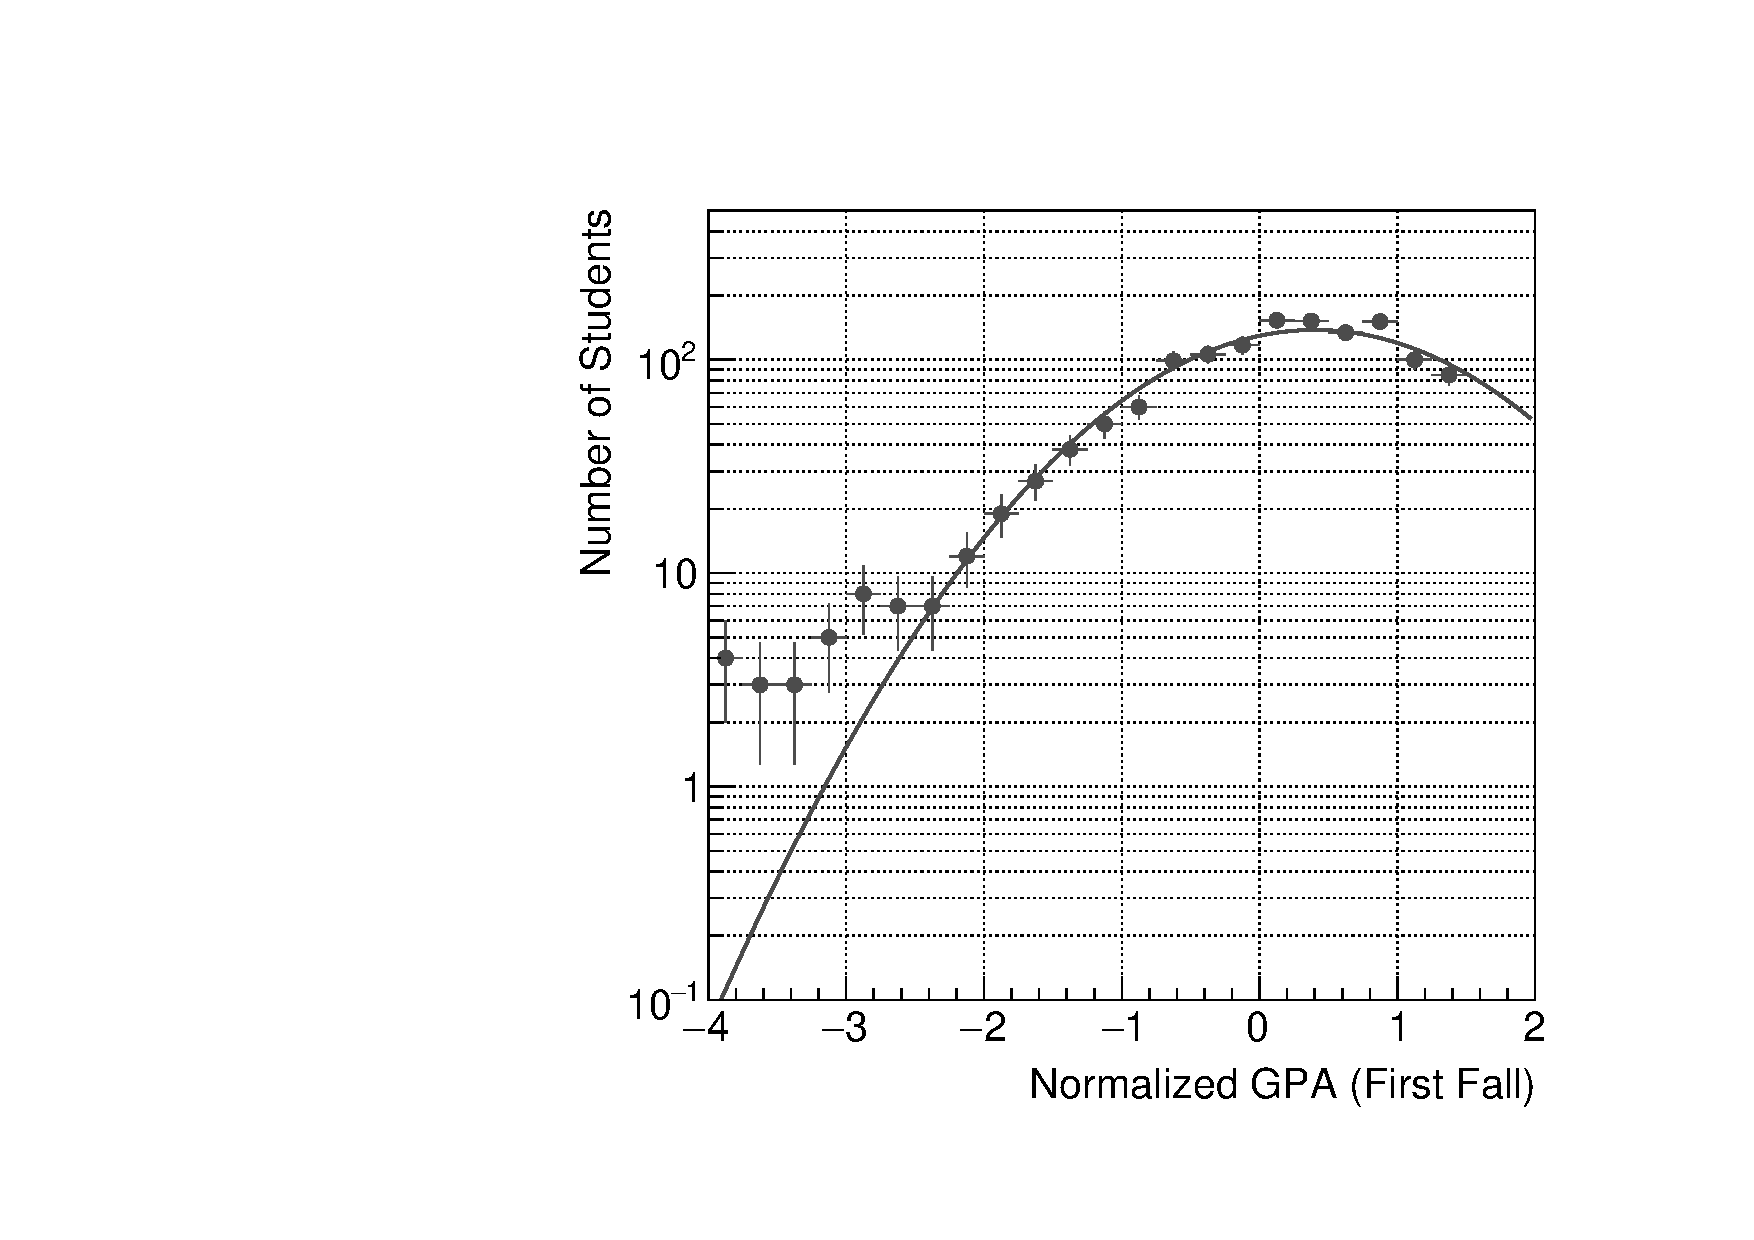
\includegraphics[width=0.4\textwidth]{figures/Nov15_plot3.pdf}
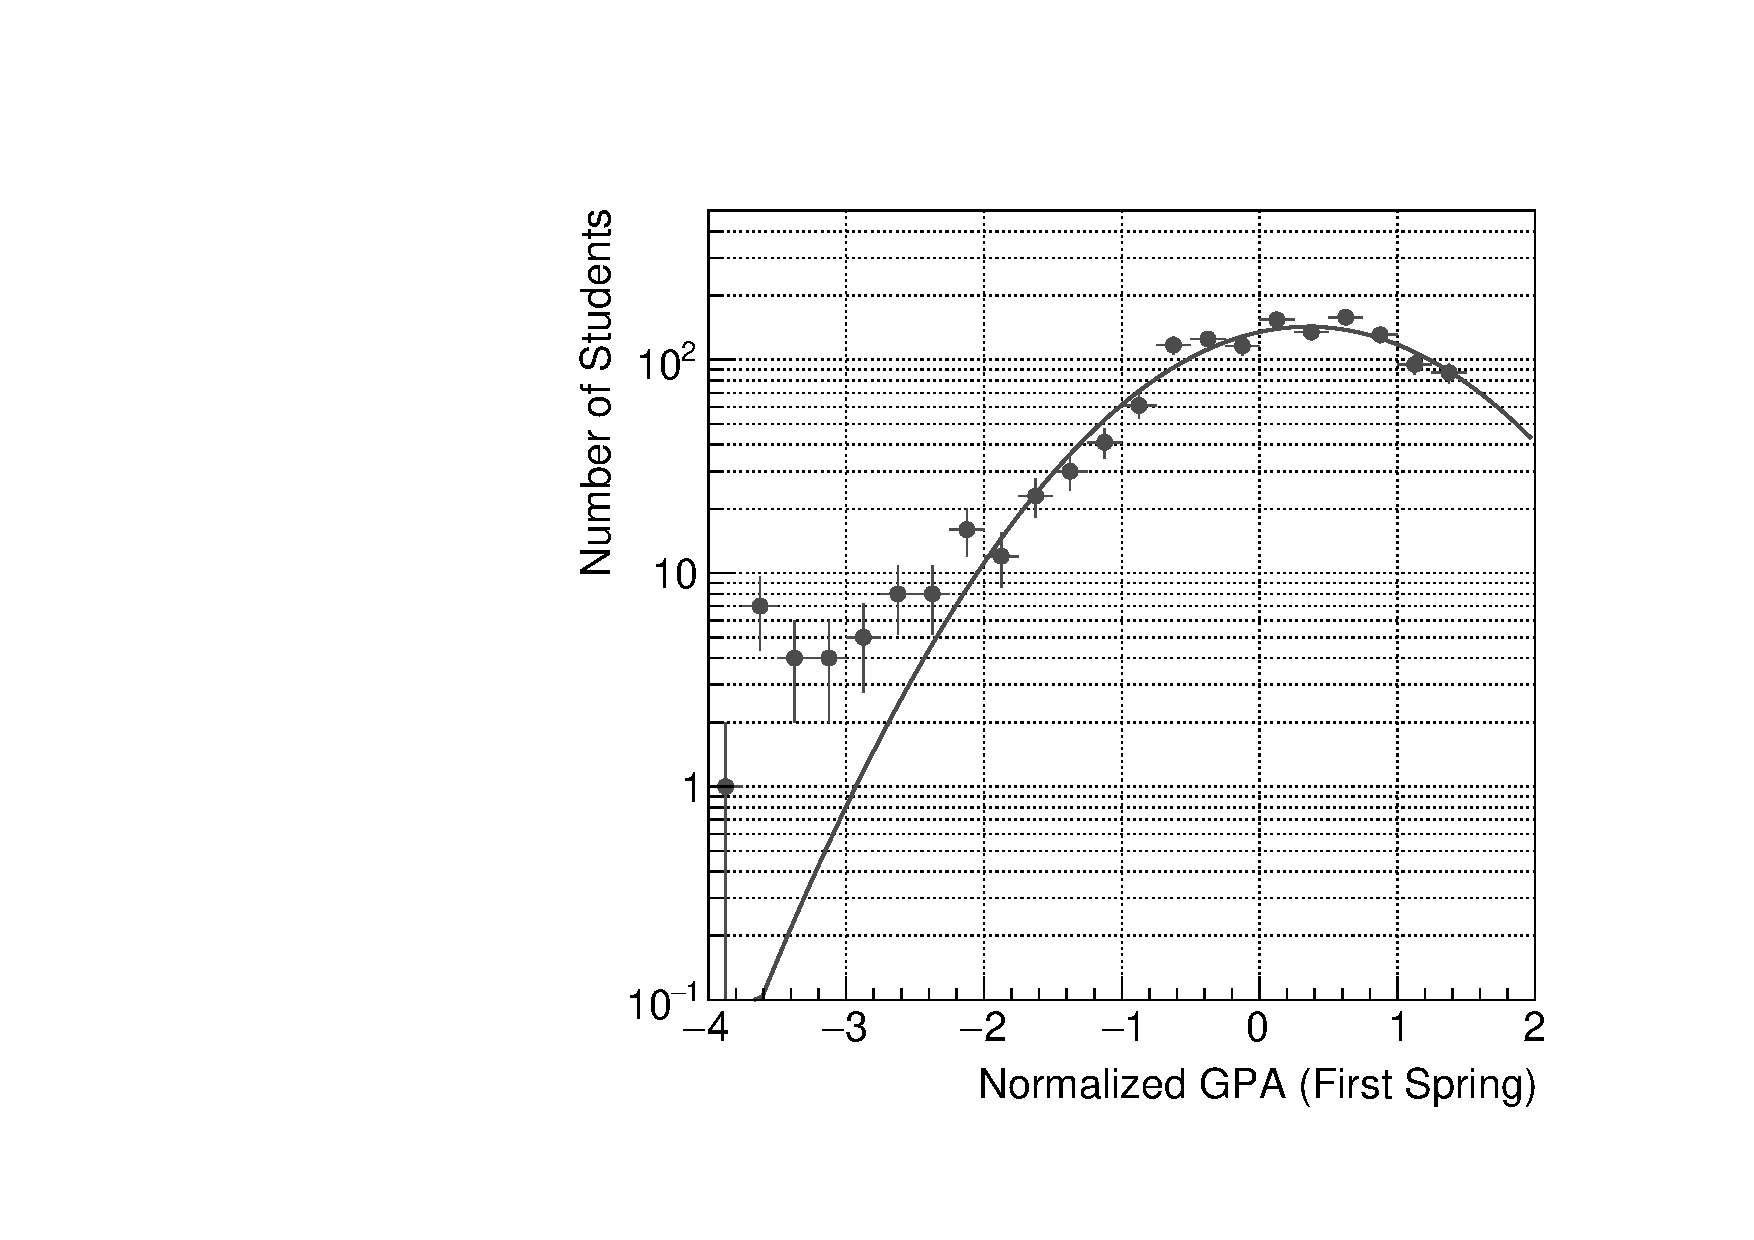
\includegraphics[width=0.4\textwidth]{figures/Nov15_plot9.pdf}
\caption{\label{fig:grade} (Left) A histogram of GPAs for 1,346 Whittier College students in the first semester.  (Right) Same, but for the second semester.}
\end{figure}

The next step was to try and find a way to identify these students in advance using the data we had historically.  Of course, what decisions to make based on the data should always be a consensus-based discussion for the committee.  My job was to attempt to find clues as to why we observed students receiving GPS 3-4 standard deviations below the mean at a rate 10 times higher than predicted by the normal distribution.  I ran a series of statistical analyses using a software package called TMVA, which was part of the ROOT C++ framework used in particle physics (see \url{https://root.cern/}).  I found that for students that \textit{do} proceed to the sophomore year, data from high school and college, and data from the first and second semester in college, is highly correlated.  For example, the relationship between high school GPA and first semester college GPA is a tight linear correlation for students that pass to sophomore year, although they do not receive the exact same GPA in college as in high school.  For students that we knew did not proceed to sophomore year, the data yielded no strong correlations.  I tried two machine learning methods to factor the data into statistics that would reveal the difference between students that do and do not proceed.  Although the algorithms could classify the extreme cases, I felt there was too much overlap to use them effectively, and that there had to be more to the story.
\\
\vspace{0.25cm}
As part of the first analysis, I was fitting normal distributions to statistical data generated by our students.  One data column that came with the original files was named ``financial aid gap.''  As I understand it conceptually, a positive aid gap means that a student is receiving various forms of financial aid that total less than what they owe in tuition, after accounting for the expected family contribution\footnote{Falone Serna was kind enough to explain it to me in detail in my second year in ESAC, but during the first year this is essentially how I understood aid gaps.}.  I noticed that I could not explain the distribution of student financial aid gap with \textit{a single} normal distribution, and that a better fit was \textit{two normal distributions.}  Statistically speaking, this finding implies that the data sample is drawn from two populations of students.  One had an average \textit{negative financial aid gap}, and the other had an average \textit{positive financial aid gap.}  It appeared that one group was receiving aid and scholarships that exceeded their tuition, and another group was receiving less.  This was the topic of my second ESAC presentation.
\\
\vspace{0.25cm}

I was able to show that aid gap is predicted by many things.  If a student has an SAT score (in any category) that is 1.5 standard deviations below the mean (or lower), then that student is almost always in the positive aid gap group.  The same is true for first and second semester GPAs.  What struck me the most was that if I graphed the aid gap distribution for just the students who did not proceed with sophomore year, a large fraction of those students were in the positive aid gap group (receiving less).  It is worth pointing out that the impetus for the analysis in the first place was Fig. \ref{fig:grade}.  Figure \ref{fig:grade2} contains the aid gap distribution.  What if the positive aid gap group and the low Whittier College GPA group were connected?  Figure \ref{fig:grade2} contains evidence of this.  However, I note that the data can be messy, and the proper claim is not simply that positive aid gap leads to low GPAs.

\begin{figure}
\centering
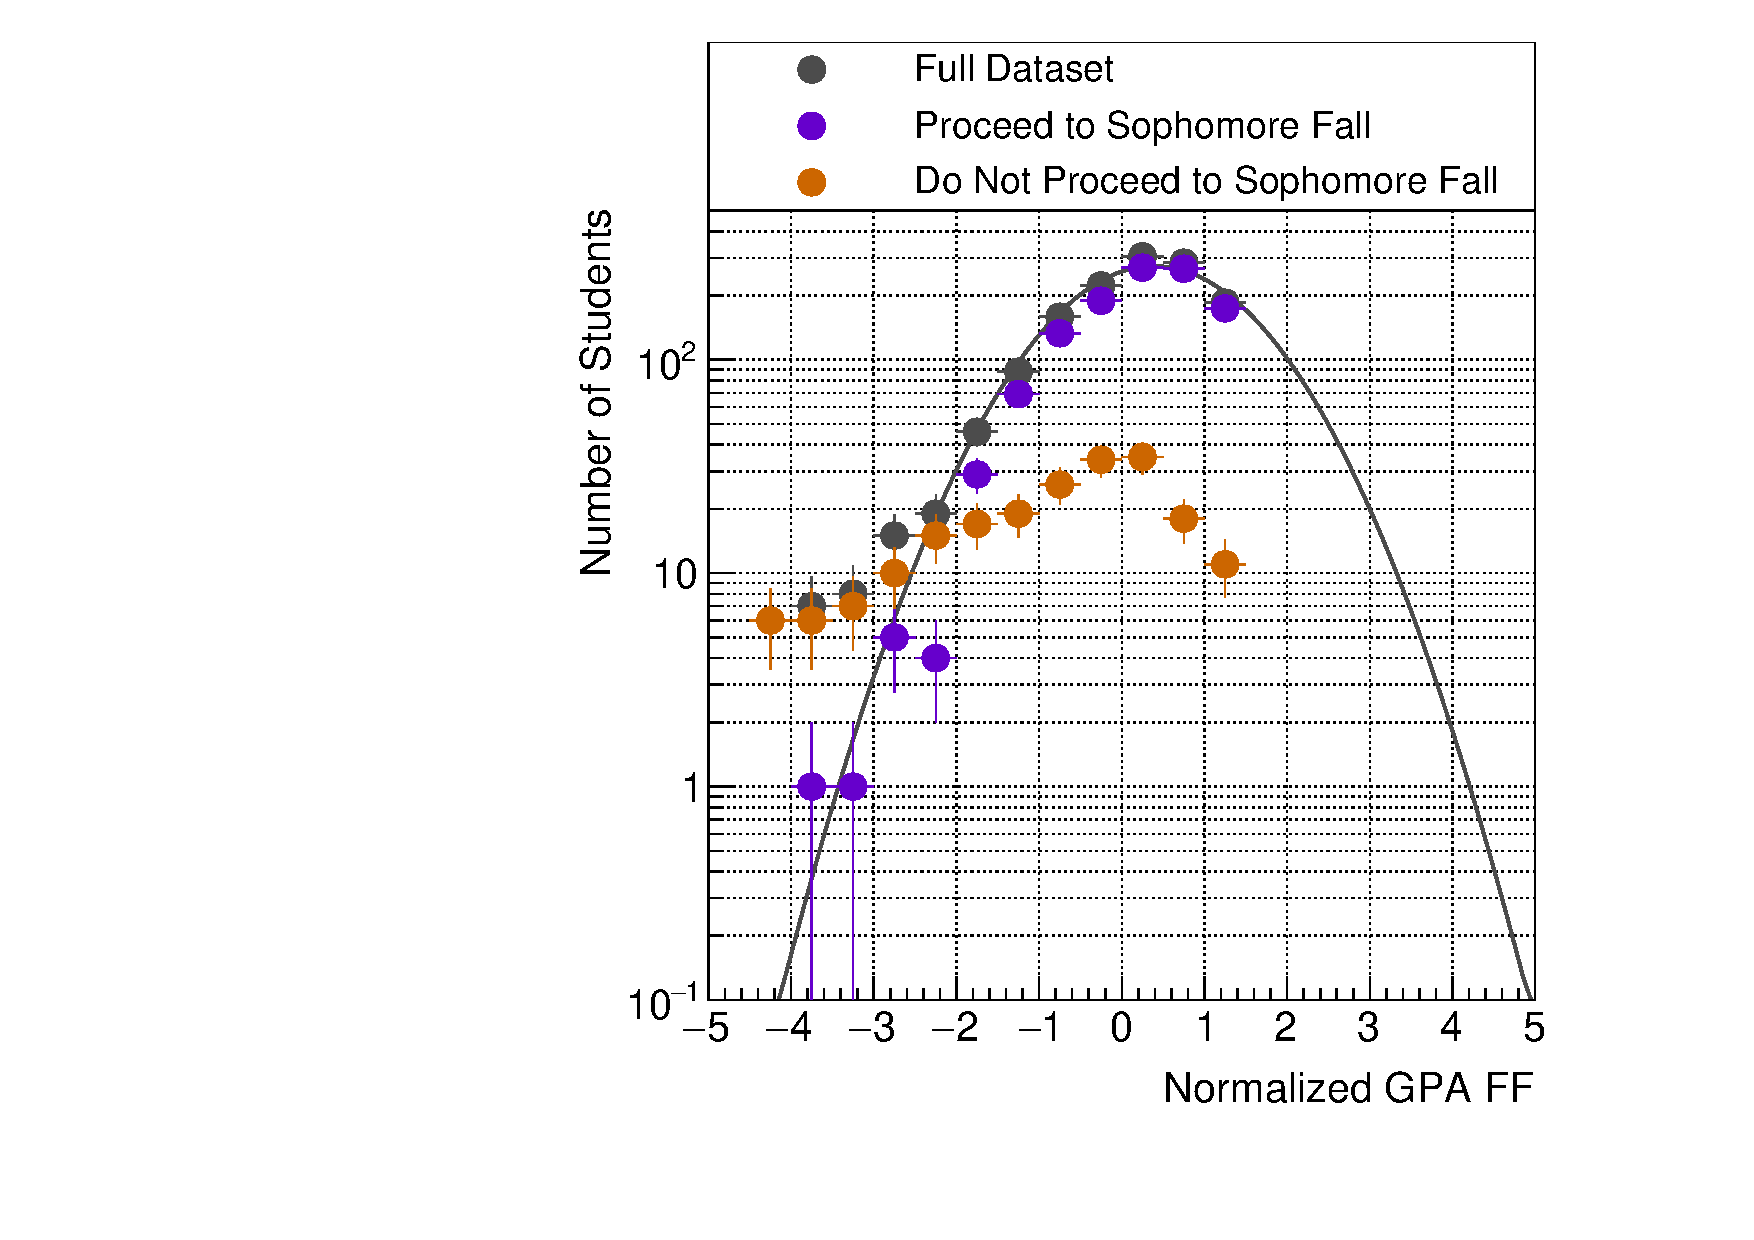
\includegraphics[width=0.4\textwidth]{figures/Dec5_plot6.pdf}
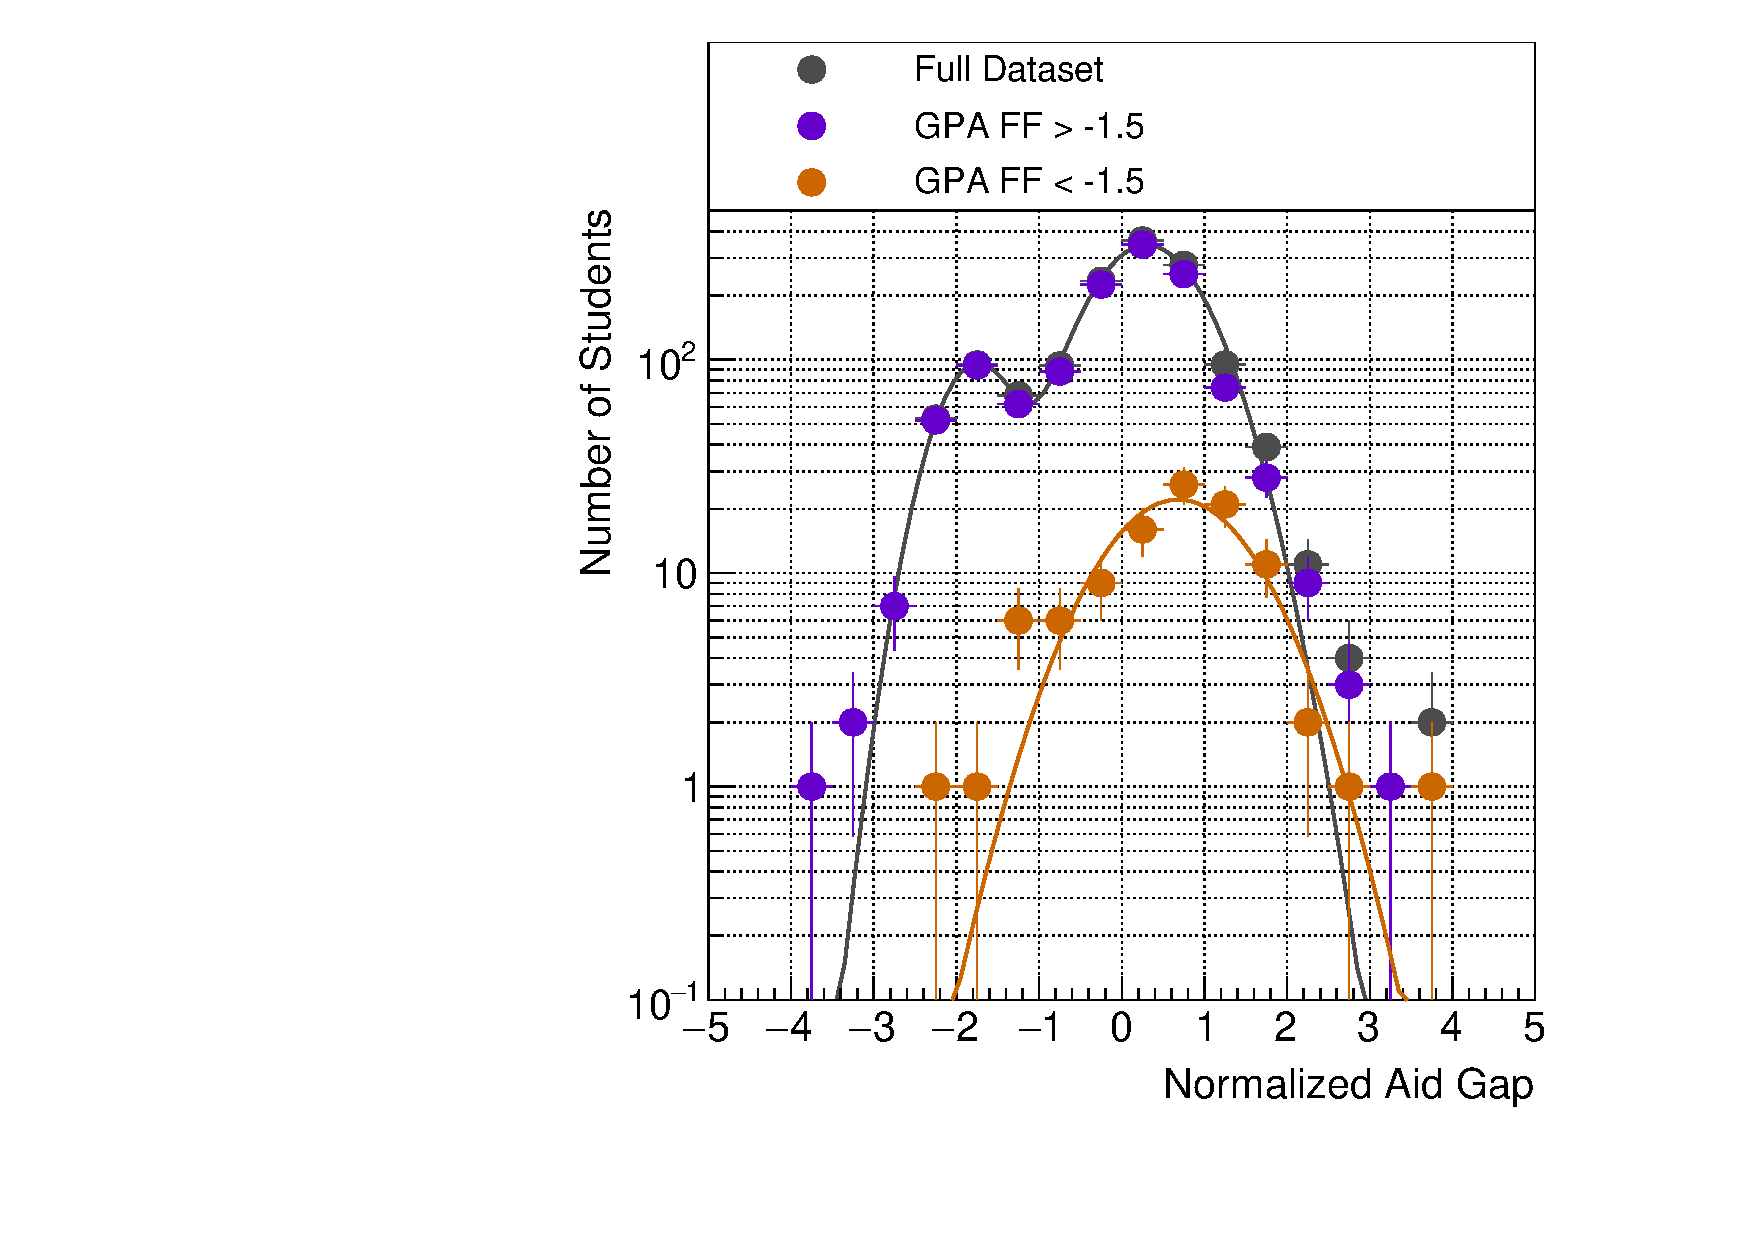
\includegraphics[width=0.4\textwidth]{figures/Dec4_plot5.pdf}
\caption{\label{fig:grade2} (Left) Histogram of normalized GPA for students' first fall semester for all students (black), those that proceed to sophomore year (purple), and those that do not (orange).  (Right) Same color scheme as (Left), but for aid gap.}
\end{figure}

Write about how I learned about orientation issues from these meetings Interactions with Falone Serna

\subsection{Educational Resources and Digital Liberal Arts Committee}

Creation of senior thesis archival program

\subsection{Whittier Scholars Program Advisory Board}

I was invited!  Sort of.

\end{document}
